%!TEX root = ../../report.tex

\subsection{Predicting with Markov model}

A use for the dynamic information is to improve the prediction of the occupancy of a cell. The prediction mechanism used with PMAC is based on an estimated occupancy value. This value is determined through the update-predict method described in section \vref{sec:cost_interpretation_path_planning}. 
In order to demonstrate the prediction, it has been used on the obstacles. The predict error score is calculated by equation \ref{eq:predict_error_score}. This is calculated for a region of interest around the obstacle position. The number of cells used in the calculation is the number of cell in the region for which the new observation has information. 

\begin{equation}
	Error_{score} = \frac{\sum\limits_{i=1}^{n_{cells}} (p_{predict}(i)-p_{observation}(i))^2}{n_{cells}}
	\label{eq:predict_error_score}
\end{equation} 

In the test only one in every fifth observations were used in the update of the current estimate in order to allow the prediction to engage. All observations were, however, used in the learning of Markov parameters. Figure \ref{fig:markov_predict_obst_2} shows the resulting score for PMAC and a simple previous prediction. The previous predictor uses the last observation as predictor, with the same one in five observations added. The score values are rather small due to the fact that the region of interest also contains static free cells which neither predictor has any trouble with. As PMAC is not initialized with any information on the dynamics these are learned through the observations. 
It is seen that the PMAC predictor does a better job at predicting the occupancy state for this obstacle. 
This is confirmed with the one-sided Wilcoxon Rang-Sum test that shows a smaller prediction error when using the PMAC predictor with $p<0.001$.
The effect of using the PMAC will vary for different obstacles. For the obstacles with low transition probabilities using the previous observation as predictor can outperform PMAC, especially if PMAC has not learned the Markov parameters accurately. 

\begin{figure}[htbp]
	\centering
	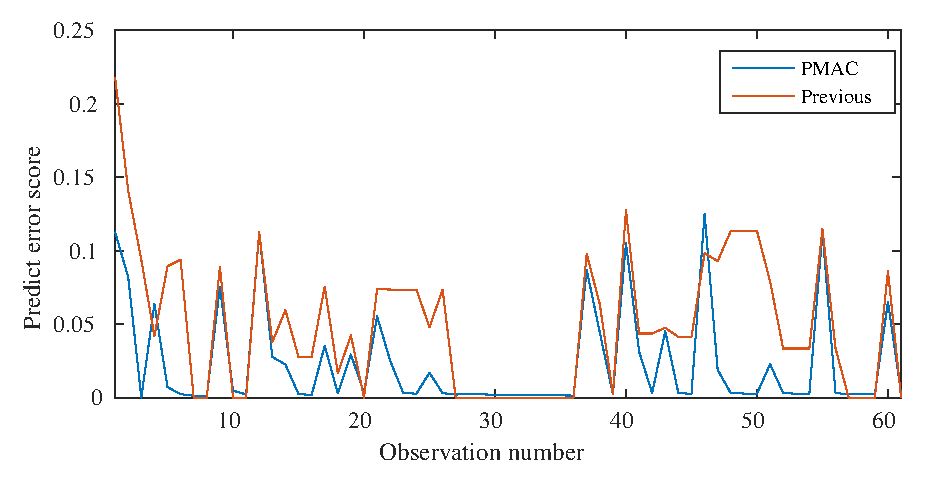
\includegraphics[scale=1]{chapters/evaluation/figures/markov_predict_figs/obstacle2_low.eps}
	\caption{Predict error score for obstacle number 2}
	\label{fig:markov_predict_obst_2}
\end{figure}%\rowcolor[gray]{0.925}

An overview of the results of the PMAC and previous observation predictor for all obstacles is shown in table \ref{table:predict_results}. It should be noted that obstacle number five has no results due to a lack of observations. The scores in the table is calculated as the average prediction error score for the respective predictors from observation number 30. It is chosen to base the scores on the last half of the observations to allow the PMAC to learn the dynamics. Along with both predict error scores are also shown a p-value from a one-sided Wilcoxon rank-sum test for smaller PMAC prediction error score median. The PMAC is successful in achieving a lower median, with p-values below 0.05, for obstacles one, seven, eight and nine. This is achieved despite the learned Markov parameters, as shown in figures \ref{fig:compare_learned_markov_entry} and  \ref{fig:compare_learned_markov_exit}, being subject to errors. It was expected that for obstacles with large Markov parameter values PMAC would perform better than the simple previous observation predictor. This is observed in the fact that three of the four obstacles where PMAC performed best, also make up the top three largest \(\lambda_{exit}\) values. The same situation is not observed in \(\lambda_{entry}\), possibly due to the poor learning of this parameter. For the more static obstacles, i.e. with lower \(\lambda\) values, the previous observation has a better probability of matching the next one.

% Please add the following required packages to your document preamble:
% \usepackage[table,xcdraw]{xcolor}
% If you use beamer only pass "xcolor=table" option, i.e. \documentclass[xcolor=table]{beamer}
\begin{table}[htbp]
	\centering
	\label{table:predict_results}
	\begin{tabular}{llllllllll}
		\toprule
		\rowcolor[gray]{0.925} 
		\textbf{Obstacle number}                                                        & \textbf{1} & \textbf{2} & \textbf{3} & \textbf{4} & \textbf{5} & \textbf{6} & \textbf{7} & \textbf{8} & \textbf{9} \\
		\begin{tabular}[c]{@{}l@{}}Previous predict \\ error score\end{tabular} & 0.076      & 0.048      & 0.063      & 0.058      & N/A        & 0.070      & 0.106      & 0.080      & 0.127      \\
		\rowcolor[gray]{0.925}
		\begin{tabular}[c]{@{}l@{}}PMAC predict \\ error score\end{tabular}     & 0.048      & 0.024      & 0.066      & 0.111      & N/A        & 0.094      & 0.080      & 0.059      & 0.065      \\
		\begin{tabular}[c]{@{}l@{}}Wilcoxon \\ p-value\end{tabular}            & < 0.001      & 0.244      & 0.716      & 1.000          & N/A        & 0.796      & 0.032      & 0.014      & 0.014     
		\\			
		\bottomrule
	\end{tabular}
	\caption{Results of prediction from previous predictor and PMAC}
\end{table}